\section{Topologia}

Para este laboratório, teremos os seguintes dispositivos: 4 roteadores (VYOS), 3 switches (EXOS), 2 Ubuntu, 1 servidor Zabbix, 1 PC Windows e 2 VPCs, como mostrado na Figura \ref{fig:topologia}.

\begin{figure*}[t]
    \centering
    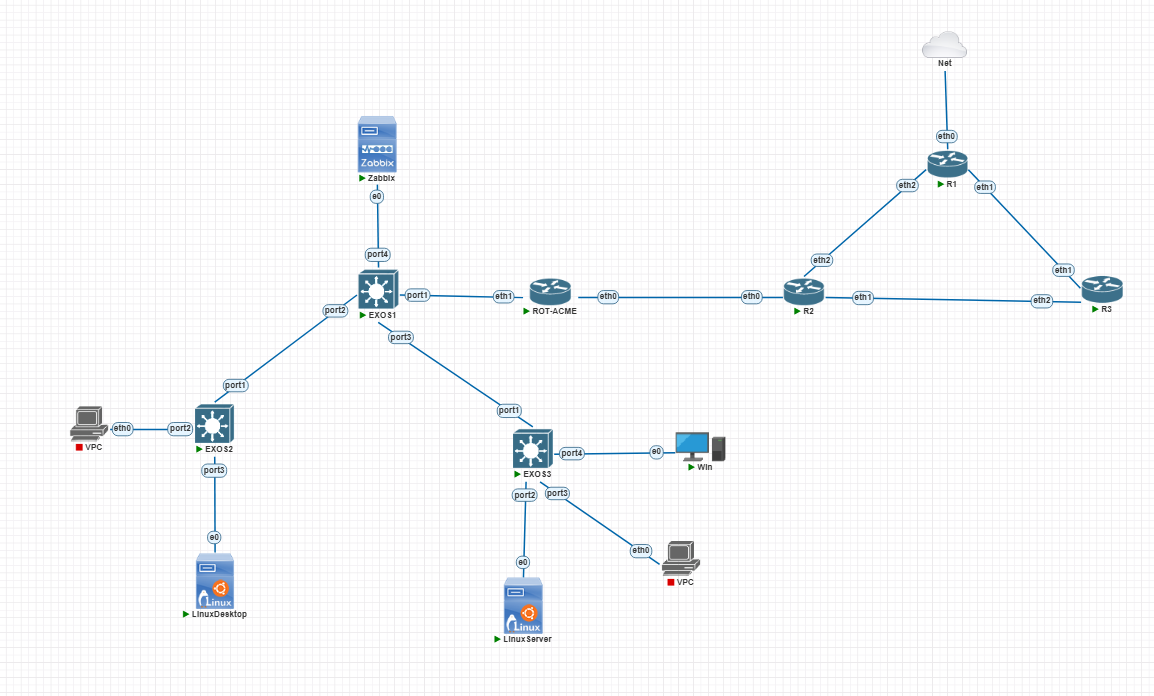
\includegraphics[width=\textwidth]{fig/topologia.png}
    \caption{Topologia}
    \label{fig:topologia}
\end{figure*}

Na Figura \ref{fig:roteadorP1}, temos os roteadores R1, R2 e R3, com a topologia em anel.

\begin{figure}[H]
    \centering
    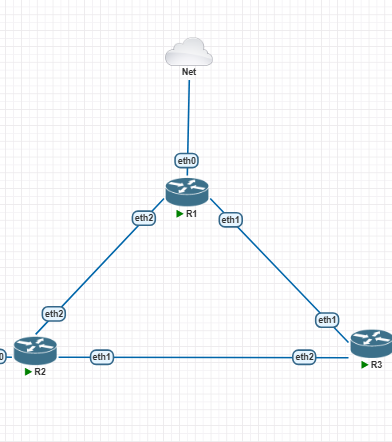
\includegraphics[width=1\linewidth]{fig/roteadorP1.png}
    \caption{Roteadores R1, R2 e R3}
    \label{fig:roteadorP1}
\end{figure}

\subsection{Roteador R1}

Para o roteador R1, temos a seguinte tabela de roteamento \ref{tab:routingR1}.

\begin{table}[h]
    \centering
    \begin{tabular}{c|c|c|c}
        Interface & Destino & Máscara \\
        \hline
        eth0 & Via DHCP & Via DHCP \\
        eth1 & 192.168.15.1 & 255.255.255.240 \\
        eth2 & 192.168.15.17 & 255.255.255.240 \\
    \end{tabular}
    \caption{Tabela de roteamento R1}
    \label{tab:routingR1}
\end{table}

\subsection{Roteador R2}

Para o roteador R2, temos a seguinte tabela de roteamento \ref{tab:routingR2}.

\begin{table}[h]
    \centering
    \begin{tabular}{c|c|c|c}
        Interface & Destino & Máscara \\
        \hline
        eth0 & 192.168.15.30 & 255.255.255.240 \\
        eth1 & 192.168.15.33 & 255.255.255.240 \\
    \end{tabular}
    \caption{Tabela de roteamento R2}
    \label{tab:routingR2}
\end{table}

\subsection{Roteador R3}

Para o roteador R3, temos a seguinte tabela de roteamento \ref{tab:routingR3}.

\begin{table}[h]
    \centering
    \begin{tabular}{c|c|c|c}
        Interface & Destino & Máscara \\
        \hline
        eth1 & 192.168.15.46 & 255.255.255.240 \\
        eth2 & 192.168.15.50 & 255.255.255.240 \\
    \end{tabular}
    \caption{Tabela de roteamento R3}
    \label{tab:routingR3}
\end{table}

\subsection{Roteador ROT-ACME}
O roteador ROT-ACME, mostrado na Figura \ref{fig:roteadorROT}, interliga a rede local com os roteadores da topologia em anel.

\begin{figure}[H]
    \centering
    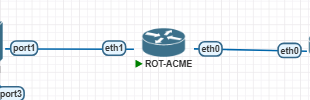
\includegraphics[width=1\linewidth]{fig/roteadorROT.png}
    \caption{Roteador ROT-ACME}
    \label{fig:roteadorROT}
\end{figure}

A Tabela \ref{tab:routingROTACME} representa a tabela de roteamento do ROT-ACME.

\begin{table}[h]
    \centering
    \begin{tabular}{c|c|c|c}
        Interface & Destino & Máscara \\
        \hline
        eth0 & 192.168.15.14 & 255.255.255.240 \\
        eth1 & 172.24.1.254 & 255.255.255.0 \\
    \end{tabular}
    \caption{Tabela de roteamento ROT-ACME}
    \label{tab:routingROTACME}
\end{table}

